Section \ref{section:related_work} has explored the K-Means clustering algorithm, its initialization techniques, approximations to enhance performance, and parallelization methods. We have examined the advantages and disadvantages of each approach and how they can be applied in various contexts. In particular, we have seen that K-means++ initialization produces better results, but requires an initial time cost, methods operating on samples of the entire dataset improve performance but decrease the quality of the results, and parallelization improves performance but does not always scale as expected due to diminishing returns. Our goal is to solve these trade-offs, and to have a method able to increase performance without sacrificing the quality of the results, and without paying an initial time-cost.  In order to accomplish this, we suggest breaking the cyclic dependency existing in K-Means, highlighted in section 2, by using Speculation. 

\subsection{Breaking K-Means dependencies}

We saw how Algorithm \ref{alg:1} consists of two main steps: the assignment step and the update step. The assignment step includes \ref{alg:step:3} and \ref{alg:step:4}, while the update step includes \ref{alg:step:5}. The two steps are dependent on each other, as the assignment of data points depends on the current cluster centers, which are in turn updated based on the assignments. This creates a cyclical pattern in the k-means algorithm.

We can group the K-Means steps into stages, each containing an Assignment step and
an Update step. Many of these stages are repeated in the K-Means algorithm until convergence.
A first way of breaking the highlighted dependencies would be to separate in each stage the Update and Assignment into two different processes. This would allow them to run in parallel, thus reducing the overall time of execution of a stage. This could be done by speculating the result of the Assignment (or the Update) allowing the consequent Update (or the Assignment) to start running concurrently. Finally, we could perform a repair step once the correct result of the Assignment (or the Update) is available. Repeating this process until convergence would result in a faster K-Means algorithm.

However, after a study of the time of executions, we can see how the Assignment step takes more time than the Update step. In particular, the ratio between the time of an Assignment step and the time of the Update step increases with $k$, as shown in Figure \ref{fig:ratio_k}. As consequence, the parallelization of Assignment and Update in each stage results inefficient, since the gain of the concurrent execution is irrelevant for $t_{Assignment} \gg t_{Update}$.

\begin{figure}[h]
\centering
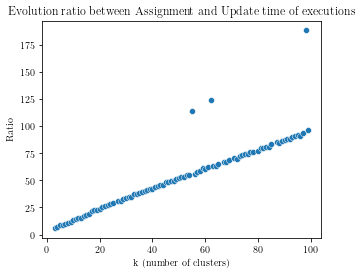
\includegraphics[width=\linewidth]{./plots/ratio_k.png}
\caption{Evolution of ratio between time execution of Assignment and Update}
\label{fig:ratio_k}
\end{figure}

Therefore, we decided to use a different approach in the implementation of Speculation. Instead of running Assignment and Update in parallel for each stage, we run two executions of K-Means concurrently. Both executions start with the same given centroids, but there are two distinct executions: the slow execution, which processes one stage consisting of one Assignment step and one Update step using the full dataset, and the fast execution, which runs on a sample of the dataset and is able to process multiple stages in the same amount of time as the slow execution. As soon as the slow execution finishes, the fast execution is interrupted, to guarantee that they both to take the same amount of time.
Finally, we compare the centroids proposed by both the executions, we compute the inertia they lead to on the entire dataset, and we pick the centroids with the smallest inertia.
\begin{algorithm}
\caption{K-Means Clustering using Speculation}
\label{alg:kmeans_speculation}
\begin{algorithmic}[1]
\State Initialize centroids $c_i$ randomly
\State Create two threads of execution: slow and fast
\label{state:create_threads}
\State Run 1 Assignment step and 1 Update step on the slow execution starting from $c_i$
\State Run as many as possible steps on a sample of the dataset on the fast execution starting from $c_i$
\State When slow execution finishes, stop fast execution. Get the proposed centroids $c_{slow}$, $c_{fast}$
\State Compute the inertia $I_X(c_{slow})$, $I_X(c_{fast})$ on the entire dataset $X$
\State $c_i = argmin_c(I_X(c_{slow}), I_X(c_{fast}))$ select centroids minimizing the inertia.
\label{state:select_centroids}
\While{not (centroids no longer move | a maximum number of iterations is reached)}
    \State repeat \ref{state:create_threads} to \ref{state:select_centroids}
\EndWhile
\State Return the final clusters and centroids
\end{algorithmic}
\end{algorithm}

The fast execution of the K-Means algorithm is used to speculate and predict future centroids that the slow execution may encounter, by traversing a speculative path, where it predicts which are going to be the results of the future stages of the slow execution. In case its prediction is correct, it will allow skipping several steps of the K-Means algorithm, breaking this way the cyclic dependency. This is possible since it works on a subset of the dataset, allowing it to execute faster and dive deeper into the algorithm, approaching more the convergence. However, as discussed in Section \ref{section:approximation}, this comes at a cost since, the fast execution is working on a subset of the dataset, therefore the final solution may not be as accurate. To avoid this, the slow execution is used to compute the result on the entire dataset, ensuring an accurate final result. Thus, the two executions have different purposes, with the fast execution being used to speculate and the slow execution being used to ensure accuracy.

In Figure \ref{fig:speculation_conceptual_design},we illustrate the proposed design. We indicate the Assignment step with $A$ and the Update step with $B$. The green shapes represent the steps actually executed, whereas the red ones indicate the steps we would save in case the speculation of the fast execution is correct. 

\begin{figure}[h]
\centering
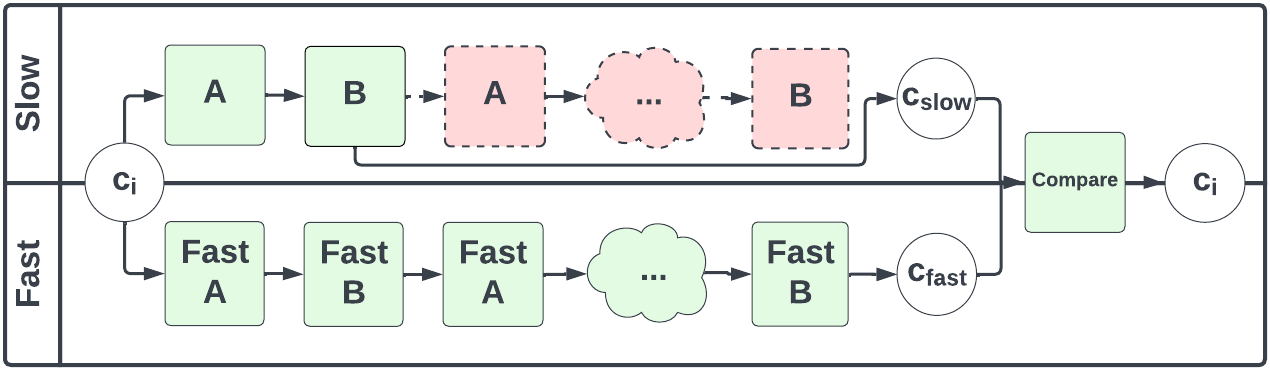
\includegraphics[width=\linewidth]{./plots/speculative_KMeans_conceptual_design.png}
\caption{Conceptual Design of Speculative K-Means}
\label{fig:speculation_conceptual_design}
\end{figure}


\subsection{Escaping local minima}

As we saw in Section \ref{alg:K-Means_pp_initialization}, it is important to note how important the initialization is in K-Means, as it determines the quality of the final clustering. K-Means++ improves the final results, but has an initial-time cost. We propose an alternative approach that avoids this cost, while still leading to a global minimum.

Figure \ref{fig:speculation_conceptual_design} and Algorithm \ref{alg:kmeans_speculation} show how the fast execution starts from the same centroids as the slow execution. However, by doing this, both executions are conditioned by the first initialization of the centroids. We suggest that the fast execution starts from a slightly different set of centroids than the slow one. This would allow us to take advantage of the fast execution to explore more of the solution space, searching for global minima.  At the same time, the repair step, where we compare the found centroids by computing their inertia, will guarantee convergence. This method is similar to having a vanilla K-Means executed many times from different initial centroids, and picking the best-obtained solution, but it is implemented only on the fast execution.

Each time we start the speculation phase, we suggest sampling $k$ datapoints from the dataset as new initial centroids $c_i'$, and modifying the starting centroids of the fast execution by combining linearly the given initial centroids and the sampled ones
\begin{equation}
c_i = p \cdot c_i' + (1-p) \cdot c_i
\end{equation} The value $p$ determines how intensely we want to perturb the initial centroids: the closer it is to $1$ the more random the centroids are, and the more we explore the solution space. This parameter expresses the degree of exploration we want from the fast execution. It can be set statically before the K-Means execution to an optimal value which may vary from dataset to dataset, or it can be adapted at run time, by adapting the randomness based on the quality of solutions we are finding stage after stage.
